\chapter{\selectlanguage{greek}Μέθοδοι προσομοίωσης}
Κεφάλαια 3 και 4
\begin{itemize}
\item Αποτέλεσμα και σχόλια
\item Περιγραφή του \en{CST Particle Studio}
\item \en{Screenshots}
\end{itemize}
Στο κεφάλαιο αυτό περιγράφεται η υλοποίηση του συστήματος, με βάση
τη μελέτη που παρουσιάστηκε στο προηγούμενο κεφάλαιο. Αρχικά
παρουσιάζεται η πλατφόρμα και τα προγραμματιστικά εργαλεία που
χρησιμοποιήθηκαν. Στη συνέχεια δίνονται οι λεπτομέρειες υλοποίησης
για τους βασικούς αλγορίθμους του συστήματος καθώς και η δομή του
κώδικα.

\begin{enumerate}
	\item \en{Directory $``$Static beam$"$}. Από \cite{Logatchov1999} έχουμε τις σχέσεις 
		\begin{equation}
			\theta_y (x) = \frac{2 \rho r_e}{\beta} \int_{-\infty}^{\infty}\frac{n(z) \dd z}{\rho^2 + \left(x+\beta z \right) ^2}
		\end{equation}
		\begin{equation}
			\theta_z(x) = 2 r_e \int_{-\infty}^{\infty}\frac{(x+\beta z)n(z) \dd z}{\rho^2 + \left(x+\beta z \right) ^2}
		\end{equation}
		Αυτά τα κάνουμε \en{plot} και είδαμε πώς επηρεάζονται από 
		\begin{itemize}
			\item \en{bunch intensity}
			\item \en{bunch length}
			\item \en{Y-offset} ($\rho$) 
			\item \en{probe beam voltage} 
		\end{itemize}   
\end{enumerate}

\section{\selectlanguage{greek}Προσομοίωση με το \en{CST Particle Studio}}
Το \en{CST Particle Studio} μπλα μπλα μπλα.

\section{\selectlanguage{greek}Προσομοίωση με το \en{CST Particle Studio} και το \en{MATLAB}}

\section{Επιρροή διάφορων μεταβλητών σε έναν \en{Electron Beam Scanner}}
Όπως περιγράφεται και  Από \cite{Logatchov1999} έχουμε τις σχέσεις 

\en{The thin probe beam moves along $X$ axis, is orthogonal to the direction of the relativistic bunch motion ($Z$ axis) with the offset parameter $\rho$ (Fig.1).}
%TODO extract figure 1 from Logatchov1999
\en{The results of scanning are monitored on the screen parallel to the $Y-Z$ plane and positioned at the distance $L$ from $Z$ axis. 
Let the center of the relativistic bunch is located at the origin at time $t=0$ whereas the testing beam has the uniform density along $X$ and the diameter $d \ll \rho$. 
Here, we assume $\rho$ exceeds the typical
transverse size of the relativistic bunch. 
At the time $t=0$ every testing beam particle is corresponded to the certain $x$-coordinate. 
The total deflecting angle in $Y$ direction for every particle under the influence of the electric field of the relativistic bunch can be expressed as:}
		\begin{equation}
			\theta_y (x) = \frac{2 \rho r_e}{\beta} \int_{-\infty}^{\infty}\frac{n(z) \dd z}{\rho^2 + \left(x+\beta z \right) ^2}
		\end{equation}
where $r_e$ is the classical electron radius, $\beta =v_t/c$ - the relative velocity of the testing beam, $c$ - the velocity of light, $x$ - the coordinate of testing beam particle at $t=0$, $n(z)$ - the relativistic bunch linear density along $Z$ axis. 
The expression for the deflecting angle of the particle
in $Z$ direction due to magnetic field can be written as:		
		
		\begin{equation}
			\theta_z(x) = 2 r_e \int_{-\infty}^{\infty}\frac{(x+\beta z)n(z) \dd z}{\rho^2 + \left(x+\beta z \right) ^2}
		\end{equation}
		Αυτά τα κάνουμε \en{plot} και είδαμε πώς επηρεάζονται από 
		\begin{itemize}
			\item \en{bunch intensity}
			\item \en{bunch length}
			\item \en{Y-offset} ($\rho$) 
			\item \en{probe beam voltage} 
		\end{itemize}   



\begin{figure}[tbh]
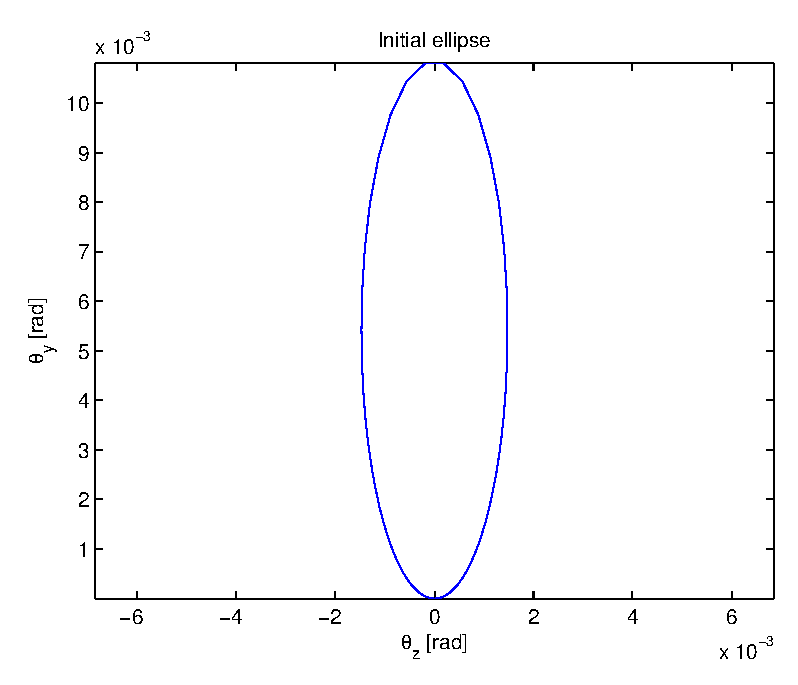
\includegraphics{figures/beam_deflection_script_01_initial_elipse}
\centering
\caption{\en{beam deflection script 01 initial elipse}}
\label{fig:beam_deflection_script_01_initial_elipse}
\end{figure}

\begin{figure}[tbh]
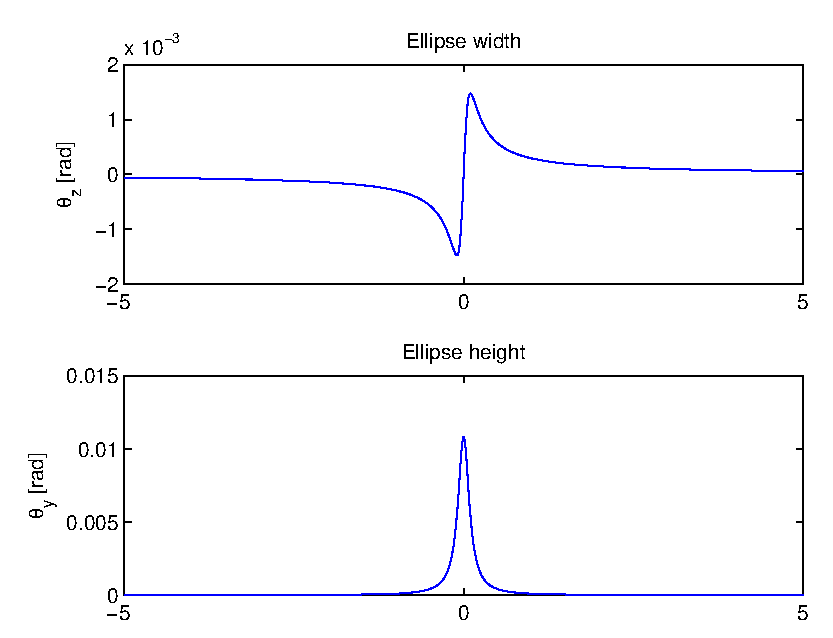
\includegraphics{figures/beam_deflection_script_02_elipse_width}
\centering
\caption{\en{beam deflection script 02 elipse width}}
\label{fig:beam_deflection_script_02_elipse_width}
\end{figure}

\begin{figure}[tbh]
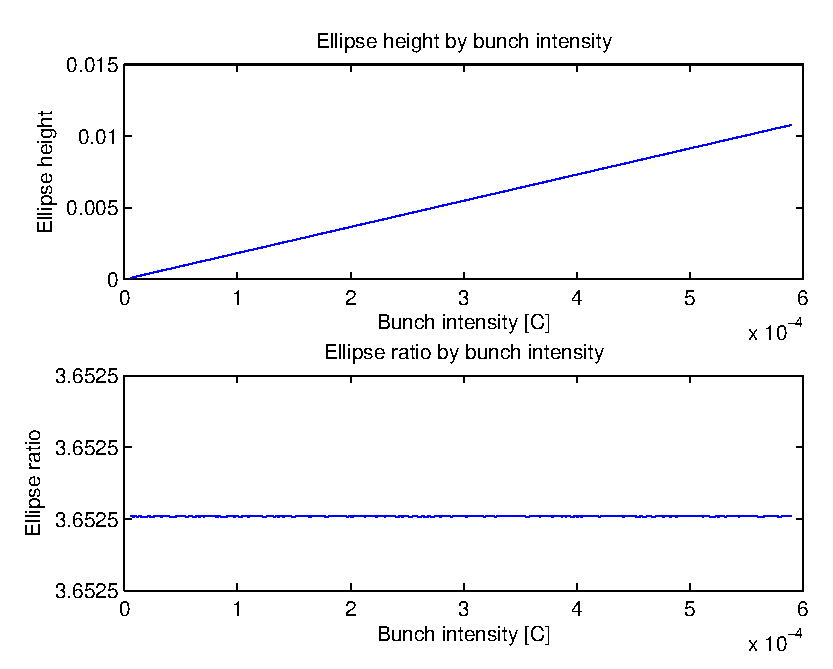
\includegraphics{figures/beam_deflection_script_03_elipse_height}
\centering
\caption{\en{beam deflection script 03 elipse height}}
\label{fig:beam_deflection_script_03_elipse_height}
\end{figure}

\begin{figure}[tbh]
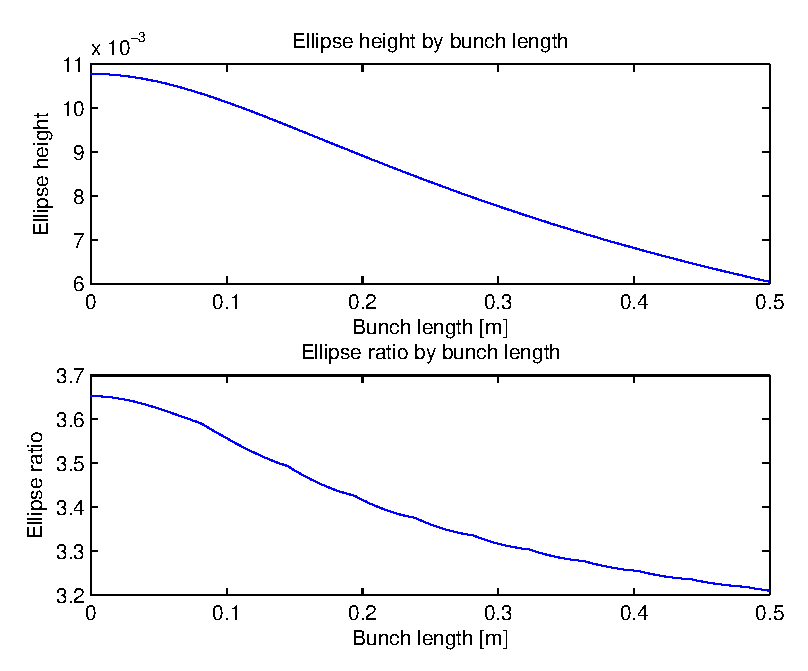
\includegraphics{figures/beam_deflection_script_04_elipse_height_by_bunch_intensity}
\centering
\caption{\en{beam deflection script 04 elipse height by bunch intensity}}
\label{fig:beam_deflection_script_04_elipse_height_by_bunch_intensity}
\end{figure}

\begin{figure}[tbh]
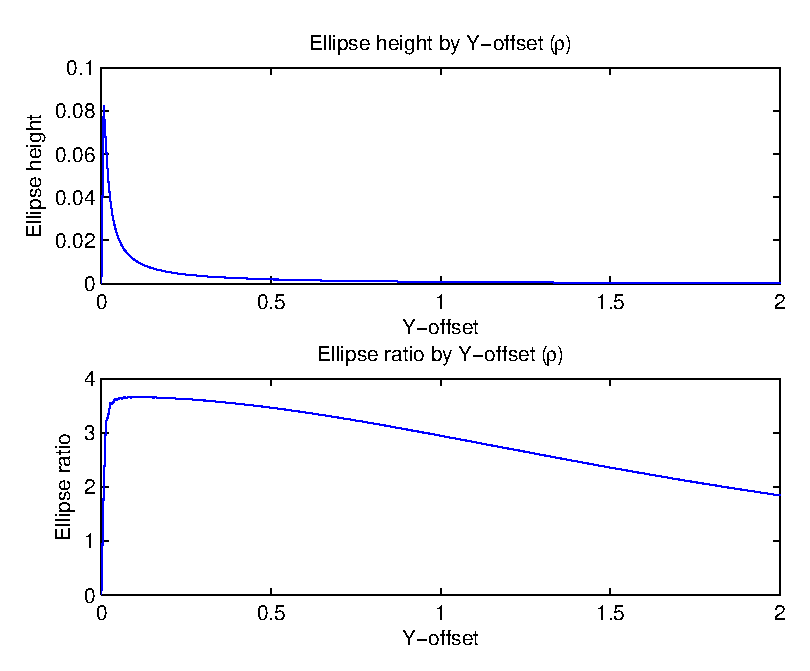
\includegraphics{figures/beam_deflection_script_05_elipse_ratio_by_bunch_intensity}
\centering
\caption{\en{beam deflection script 05 elipse ratio by bunch intensity}}
\label{fig:beam_deflection_script_05_elipse_ratio_by_bunch_intensity}
\end{figure}

\begin{figure}[tbh]
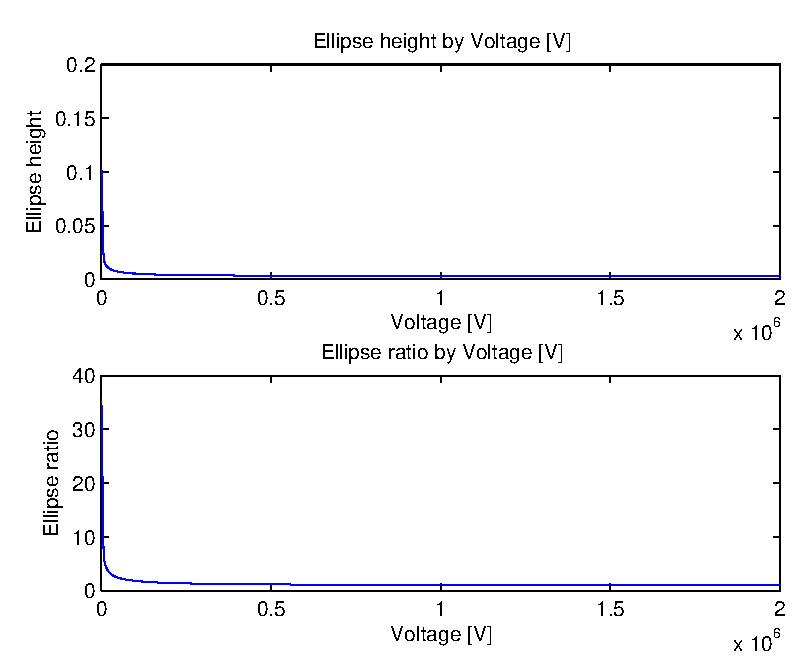
\includegraphics{figures/beam_deflection_script_06}
\centering
\caption{\en{beam deflection script 06}}
\label{fig:beam_deflection_script_06}
\end{figure}

\begin{figure}[tbh]
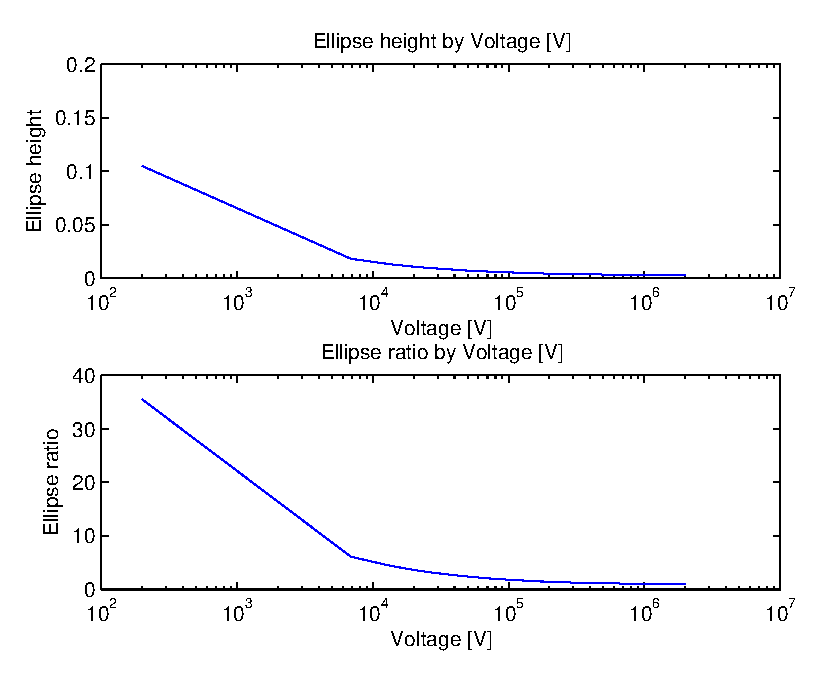
\includegraphics{figures/beam_deflection_script_07}
\centering
\caption{\en{beam deflection script 07}}
\label{fig:beam_deflection_script_07}
\end{figure}